%!TEX root = paper.tex

\newcommand{\colalg}{{\tt ColAlg}}
\newcommand{\expthree}{{\tt Exp3}}
\newcommand{\latentranker}{{\tt LRA}}
\newcommand{\rowalg}{{\tt RowAlg}}
\newcommand{\ucb}{{\tt UCB1}}

We propose \emph{latent ranker algorithm ($\latentranker$)} for solving the personalized ranking problem. The pseudocode of $\latentranker$ is in \cref{alg:latent ranker}. $\latentranker$ has two main components, column learning and row ranking.

The column learning algorithm recommends a list of $d$ columns and is the same as in \citet{radlinski2008learning}. But we exploit an additional structure in our problem to show that we learn the optimal columns $J_\ast$. The column learning algorithm are $d$ instances of multi-armed bandit algorithms, which we denote by $\colalg(k)$ for algorithm $k \in [d]$. $\colalg(1)$ learns the most rewarding column on average, $\colalg(2)$ learns the second most rewarding column on average conditioned on the first learned column, as so on.

The row ranking algorithm permutes columns suggested by the column learning algorithm. The row learning algorithm are multiple instances of full-information setting algorithms. In particular, for each user $i \in [K]$ and each set of $d$ columns $J$, we have algorithm $\rowalg(i, J)$ with $d!$ arms, which correspond to all possible permutations of $J$. The objective of $\rowalg(i, J)$ is to learn a permutation of $J$ with the highest reward, as measured by \eqref{eq:reward}.

$\latentranker$ interacts with the environment as follows. At time $t$, a uniformly random user $i_t$ is revealed to $\latentranker$. Then, in the ascending order of $k \in [d]$, $\textrm{MAB}_k(n)$ suggests a column $\ell_{t, k}$. If $\textrm{MAB}_{k + 1}(n)$ suggests a previously suggested column in $\{\ell_{t, 1}, \dots, \ell_{t, k}\}$, then $\ell_{t, k + 1}$ is chosen uniformly at random from the remaining columns. We denote the set of $d$ selected columns by $J_t = (\ell_{t, 1}, \dots, \ell_{t, d})$. Then, the weighted majority instance $\textrm{WMA}_{i_t, J_t}(n)$, for user $i_t$ and columns $J_t$, selects a permutation $\pi_{t, i_t}$ of $J_t$.

The user is recommended the permuted list of items, $\pi_{t, i_t}(J_t)$, and LRA observes the individual rewards of all recommended items. After this, we update both column and row learning algorithms. The reward of $\textrm{MAB}_k(n)$, which selects the $k$-th column in $J_t$, is $\max_{j \in [k]} r_t(i_t, \ell_{t, j}) - \max_{j \in [k - 1]} r_t(i_t, \ell_{t, j})$. That is, the reward is the marginal gain of that column over previously chosen columns. Since LRA observes the individual rewards of all recommended items, we can compute the reward of any permutation of $J_t$ in row $i_t$. These rewards are then used to update $\textrm{WMA}_{i_t, J_t}(n)$. An illustrative diagram of the entire learning process is shown in \cref{fig:rankedbandit}.

\begin{figure}
    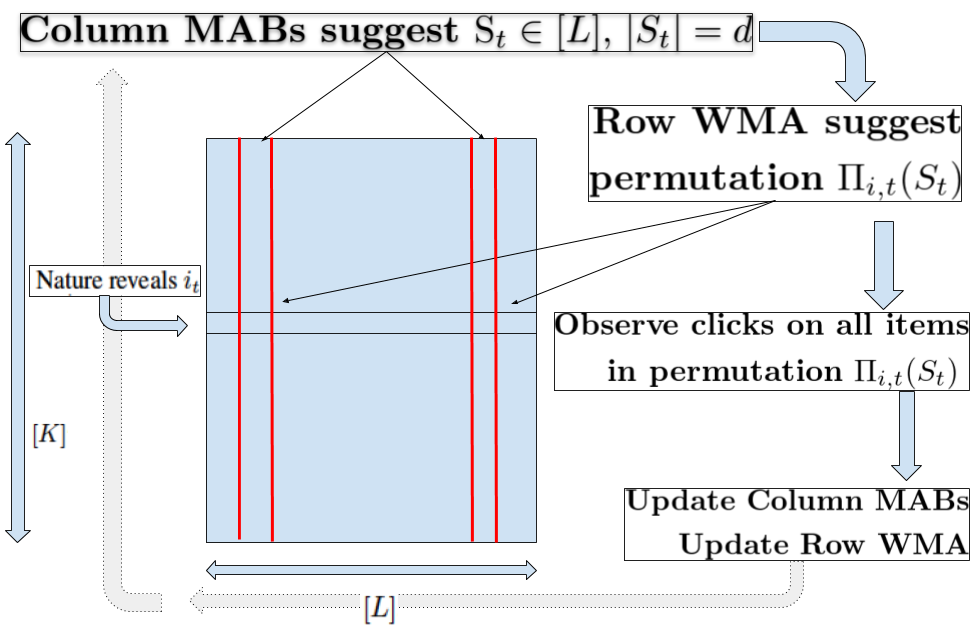
\includegraphics[scale=0.2]{img/RankedBand.png}
    \caption{Latent Ranked Bandit in rank $d=2$ scenario. \todob{The figure is super confusing. If you want to have it, add a flow chart.}}
    \label{fig:rankedbandit}
    \vspace*{-1em}
\end{figure}

\begin{algorithm}[t]
  \caption{Latent Ranker Algorithm ($\latentranker$)}
  \label{alg:latent ranker}
  \begin{algorithmic}[1]
    \State \textbf{Input:} Rank $d$, horizon $n$
    \State
    \For{$k = 1, \dots, d$}
    \Comment{Initialization}
      \State Initialize $\colalg(k)$
    \EndFor
    \ForAll{$i \in [K], J \subset [L] \text{ such that } |J| = d$}
      \State Initialize $\rowalg(i, J)$
    \EndFor
    \State
    \For{$t = 1, \dots, n$}
      \State User $i_t$ is revealed
      \For{$k = 1, \dots, d$}
      \Comment{Generate response}
        \State $\hat{\ell}_k \gets \text{ Suggested item by } \colalg(k)$
        \If{$\hat{\ell}_k \in \{\ell_1, \dots, \ell_{k - 1}\}$}
          \State $\ell_k \gets$ Random item not in $\{\ell_1, \dots, \ell_{k - 1}\}$
        \Else
          \State $\ell_k \gets \hat{\ell}_k$
        \EndIf
      \EndFor
      \State $J_t \gets (\ell_1, \dots, \ell_d)$
      \State $\pi_{t, i_t} \gets \text{ Suggested permutation by } \rowalg(i_t, J_t)$
      \State
      \State Recommend $\pi_{t, i_t}(J_t)$
      \State Observe $M_t(i_t, J_t(k))$ for all $k \in [d]$
      \State
      \For{$k = 1, \dots, d$}
      \Comment{Update statistics}
        \State Update arm $\ell_k$ of $\colalg(k)$ with reward
        \begin{align*}
          & \max \, \{M_t(i_t, J_t(a)): a \in [k]\} - {} \\
          & \max \, \{M_t(i_t, J_t(a)): a \in [k - 1]\}
        \end{align*}
        \If{$\ell_k \neq \hat{\ell}_k$}
          \State Update arm $\hat{\ell}_k$ of $\colalg(k)$ with reward $0$
        \EndIf
      \EndFor
      \ForAll{arms $\pi$ in $\rowalg(i_t, J_t)$}
        \State Update arm $\pi$ with reward $r_t(i_t, \pi(J_t))$ in \eqref{eq:reward}
      \EndFor
    \EndFor
  \end{algorithmic}
\end{algorithm}
